\documentclass[12pt,a4paper]{article}
\usepackage[a4paper, left=2.5cm,right=2.5cm,top=3cm,bottom=3cm]{geometry}
\usepackage[utf8]{inputenc}
\usepackage[spanish]{babel}
\addto\captionsspanish{
	\renewcommand\chaptername{}
	\renewcommand\appendixname{Anexo}
	\renewcommand\appendixpagename{Anexos}
	\def\tablename{Tabla}
	\def\listtablename{\'Indice de tablas}
}
\usepackage{ucs}
\usepackage{subfig}
\usepackage{float}
\usepackage{amsmath}
\usepackage{amsfonts}
\usepackage{amssymb}
\usepackage{graphicx}
\usepackage{listings}
\usepackage{color}
\usepackage[T1]{fontenc}
\usepackage[scaled]{beramono}
\usepackage{upquote}
\usepackage{xcolor}
\usepackage{listings}
\usepackage{caption}
\usepackage{subcaption}
\usepackage{chngcntr}
\usepackage{endnotes}
\usepackage{float}
\usepackage{hyperref}
\usepackage{wrapfig}
\usepackage{fancyhdr}
\usepackage{emptypage}
\usepackage{times}
\usepackage{array}
\usepackage{setspace}
\usepackage{multirow}
%\usepackage{subfigure}
\usepackage{verbatim}
%\usepackage{tabulary}
%\usepackage{graphicx,subfigure}
\usepackage[bottom]{footmisc} 
\usepackage{appendix}
\usepackage{mathtools}
\usepackage{textcomp}


%listing, code style
% Define a custom color
\definecolor{backcolour}{rgb}{0.95,0.95,0.92}
\definecolor{codegreen}{rgb}{0,0.6,0}

% Define listing style
\lstset{
	language=python,
	tabsize=4,
	rulecolor=,
	basicstyle=\scriptsize,
	upquote=true,
	aboveskip={1.2\baselineskip},
	columns=fixed,
	numbers=left,
	showstringspaces=false,
	extendedchars=true,
	breaklines=true,
	prebreak = \raisebox{0ex}[0ex][0ex]{\ensuremath{\hookleftarrow}},
	showtabs=false,
	showspaces=false,
	showstringspaces=false,
	identifierstyle=\ttfamily,
	keywordstyle=\color[rgb]{0,0,1},
	commentstyle=\color[rgb]{0.133,0.545,0.133},
	stringstyle=\color[rgb]{0.627,0.126,0.941},
} 


\renewcommand{\notesname}{Fuentes}
\renewcommand{\baselinestretch}{1.2}
\hypersetup{
	colorlinks,%
	citecolor=black,%
	filecolor=black,%
	linkcolor=black,%
	urlcolor=black
}

\begin{document}
	
\begin{titlepage}
	\centering
	%\null\vfill
	
\includegraphics[width=\textwidth]{FIGURES/Portada/Logo_portada.png} 
	\vspace{1.5cm}
	
	Universidad Politécnica de Madrid
	\\Escuela Técnica Superior de Ingeniería Aeronáutica y del Espacio
	\vspace{2cm}
	
	{\large MÁSTER UNIVERSITARIO EN SISTEMAS ESPACIALES}
	\vspace{2cm}
	
	{\LARGE MILESTONE 6}
	\vspace{1cm}
	
	{\large Ampliación de Matemáticas I}
	\vspace{4cm}
	
	\begin{center}
		\large{\textbf{\today}} \\
	\end{center}
	
	Autor: \\ Alberto García Rincón
	\vfill
\end{titlepage}

%****INDICES****
\newpage
\pagestyle{empty}
\tableofcontents	

%******DOC******	
\newpage
\pagenumbering{arabic}
\setcounter{page}{1}
\pagestyle{fancy} 

\section{Introducción} %OK
En este trabajo se ha implementado un método de resolución numérica de alto orden y de paso temporal variable. El método elegido ha sido el método ''Runge-Kutta 87''. Se ha definido también una función que define el problema restringido de los tres cuerpos. 

A continuación se han obtenido los puntos de Lagrange del sistema Tierra-Luna y se ha realizado un estudio sobre la estabilidad de dichos puntos. Finalmente se han simulado y analizado varias órbitas de un cuerpo que se encontraría en las proximidades de cada punto de Lagrange.


\section{Código de Python} %OK
\subsection{Diagrama de bloques}
\begin{figure}[H]
	\centering
	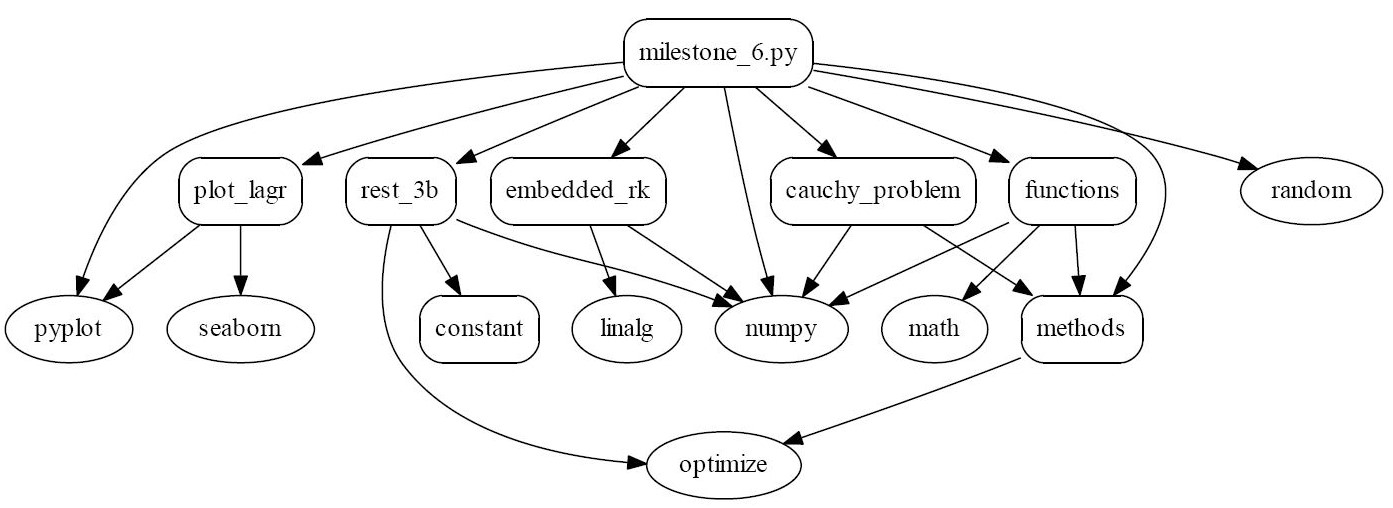
\includegraphics[width=0.99\textwidth]{FIGURES/mil6/codigo/diagrama_mil6.JPG}
	\caption{Diagrama módulos Milestone 6.}
	\label{diagram_mil6}
\end{figure}
Como puede observarse en la Figura \ref{diagram_mil6} para hacer funcionar este programa se debe ejecutar el programa principal denominado $milestone\_6.py$. Este programa se encarga de llamar al resto de funciones definidas en los respectivos archivos.

Se van a comentar las nuevas funciones implementadas para la resolución de este problema.


\subsection{milestone\_6.py}
En la Figura \ref{main1} se muestra el código que define las condiciones iniciales para realizar las simulaciones.
\begin{figure}[H]
	\centering
	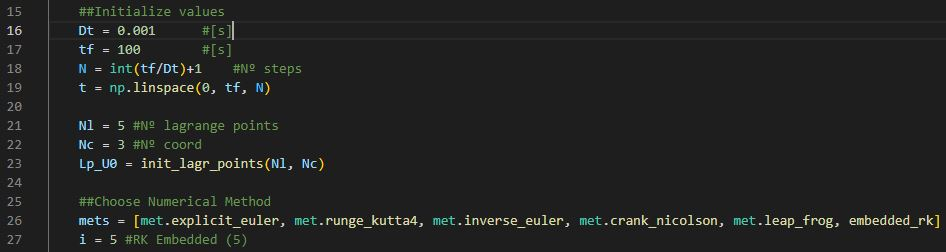
\includegraphics[width=0.95\textwidth]{FIGURES/mil6/codigo/main1.JPG}
	\caption{Condiciones iniciales Milestone 6.}
	\label{main1}
\end{figure}

En la Figura \ref{main2} se muestra el código que llama a la función encargada de determinar las coordenadas de los puntos de Lagrange del sistema Tierra-Luna definido.
\begin{figure}[H]
	\centering
	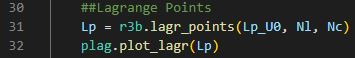
\includegraphics[width=0.7\textwidth]{FIGURES/mil6/codigo/main2.JPG}
	\caption{Código para calcular los puntos de Lagrange.}
	\label{main2}
\end{figure}

En la Figura  \ref{main3} se muestra el código que calcula una órbita en las proximidades del punto de Lagrange, lo hace para cada uno de los puntos de Lagrange calculados anteriormente. 

Se define con la función $uniform()$ un punto inicial de la órbita que se encuentra próximo al punto de Lagrange objeto de estudio. Las componentes de velocidad de ese cuerpo se inicializan en cero.
\begin{figure}[H]
	\centering
	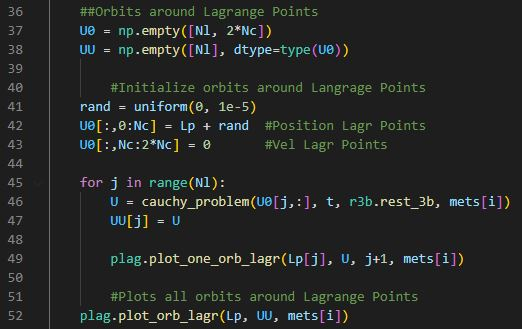
\includegraphics[width=0.7\textwidth]{FIGURES/mil6/codigo/main3.JPG}
	\caption{Código para calcular las órbitas alrededor de los puntos de Lagrange.}
	\label{main3}
\end{figure}

En la Figura \ref{main4} se muestra el código para calcular y representar los autovalores de cada punto de Lagrange.
\begin{figure}[H]
	\centering
	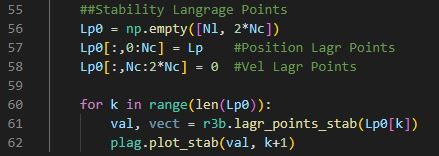
\includegraphics[width=0.7\textwidth]{FIGURES/mil6/codigo/main4.JPG}
	\caption{Código para calcular la estabilidad de los puntos de Lagrange.}
	\label{main4}
\end{figure}

\subsection{embedded\_rk.py}
Las Figuras \ref{erk1} y \ref{erk2} muestran el código del método Runge-Kutta embebido que se ha programado. 

Cabe destacar la función $step\_size()$ que define el $\Delta t$ que se va a utilizar en cada paso de la resolución del proceso. Esto es porque al tratarse de un método de paso temporal variable, es decir que el $\Delta t$ se ''autocalcula'' para cada paso del proceso.
\begin{figure}[H]
	\centering
	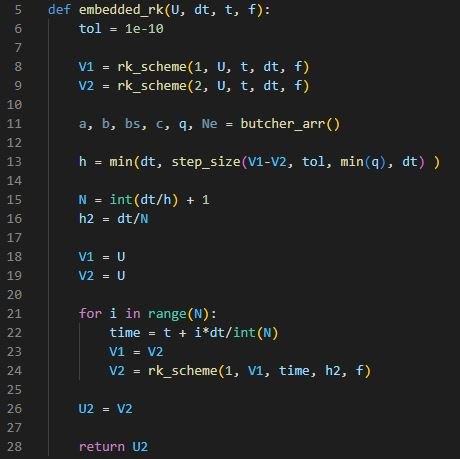
\includegraphics[width=0.7\textwidth]{FIGURES/mil6/codigo/erk1.JPG}
	\caption{Código función método numérico Runge-Kutta embebido.}
	\label{erk1}
\end{figure}
\begin{figure}[H]
	\centering
	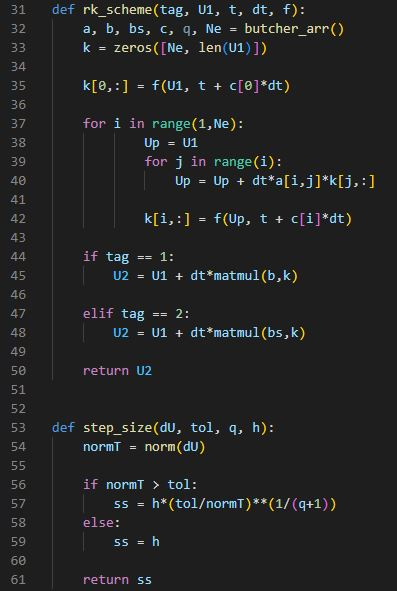
\includegraphics[width=0.7\textwidth]{FIGURES/mil6/codigo/erk2.JPG}
	\caption{Código función método numérico Runge-Kutta embebido.}
	\label{erk2}
\end{figure}

La Figura \ref{erk3} muestra el array de Butcher que se ha utilizado para el método Runge-Kutta definido anteriormente. Se trata de un método de orden 8, denominado $RK87$.
\begin{figure}[H]
	\centering
	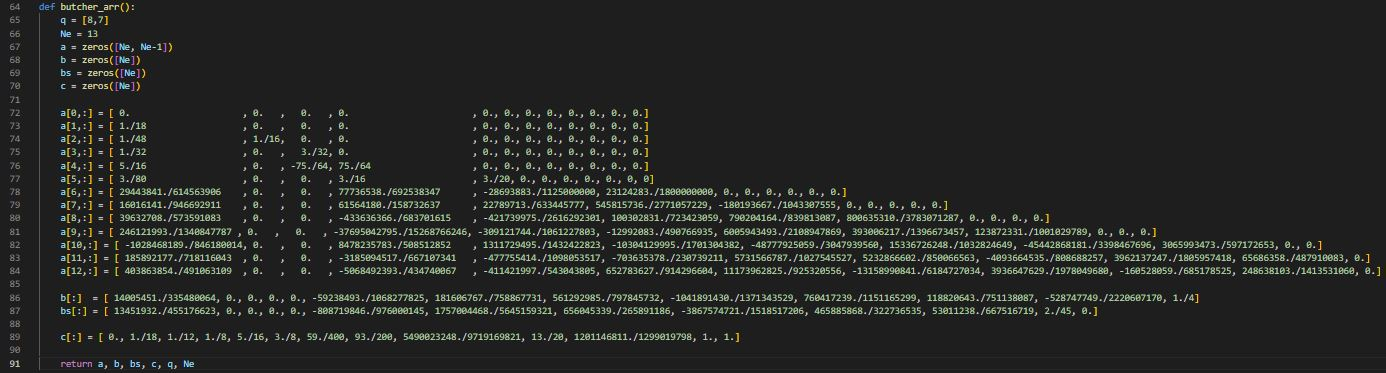
\includegraphics[width=1\textwidth]{FIGURES/mil6/codigo/erk3.JPG}
	\caption{Código función Butcher\_array.}
	\label{erk3}
\end{figure}

\subsection{rest\_3b.py}
En la Figura \ref{r3bp1} se expone el código que define el problema de los 3 cuerpos con movimiento circular restringido. Es un caso particular del problema de los N-Cuerpos que se había definido en el anterior trabajo.

Se trata de la función que se va ha utilizar para en las siguientes simulaciones. Los tres cuerpos que se integran en esta función son: la Tierra, la Luna y el tercer cuerpo es un cuerpo que se encuentra en las proximidades del punto de Lagrange objeto de estudio.

\begin{figure}[H]
	\centering
	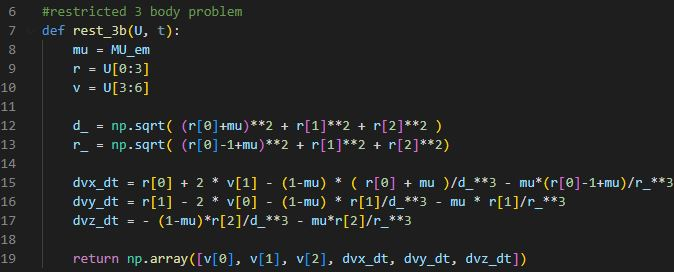
\includegraphics[width=0.85\textwidth]{FIGURES/mil6/codigo/r3bp1.JPG}
	\caption{Código función problema de los 3 cuerpos restringido con movimiento circular.}
	\label{r3bp1}
\end{figure}

La Figura \ref{r3bp2} define la función que calcula los puntos de Lagrange dados unos valores iniciales aproximados. Esta función hace uso de la función definida en \ref{r3bp1}.
\begin{figure}[H]
	\centering
	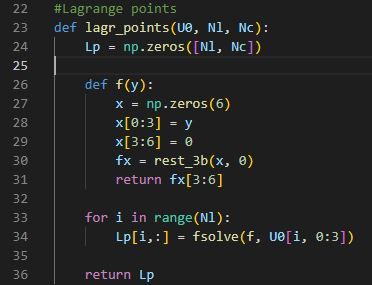
\includegraphics[width=0.7\textwidth]{FIGURES/mil6/codigo/r3bp2.JPG}
	\caption{Código función cálculo puntos de Lagrange.}
	\label{r3bp2}
\end{figure}

La Figura \ref{r3bp3} define el código necesario para el cálculo de los autovalores de las regiones de estabilidad de los puntos de Lagrange. La función $sist_matrix()$ calcula el Jacobiado asociado a cada punto que se le pasa como argumento.
Con el comando $eig(A)$ obtenemos los autovalores y los autovectores de la matriz Jacobiana.
\begin{figure}[H]
	\centering
	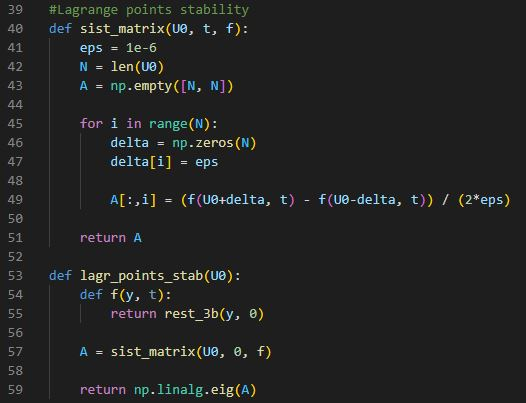
\includegraphics[width=0.7\textwidth]{FIGURES/mil6/codigo/r3bp3.JPG}
	\caption{Código funciones cálculo autovalores y autovectores de los puntos de Lagrange.}
	\label{r3bp3}
\end{figure}

\subsection{plot\_lagr.py}
La Figura \ref{plot_lagr1} muestra la función que dibuja en 3 dimensiones, puesto que los cálculos se han realizado considerando las 3 coordenadas geométricas, los puntos de Lagrange en el sistema Tierra-Luna; también representadas.
\begin{figure}[H]
	\centering
	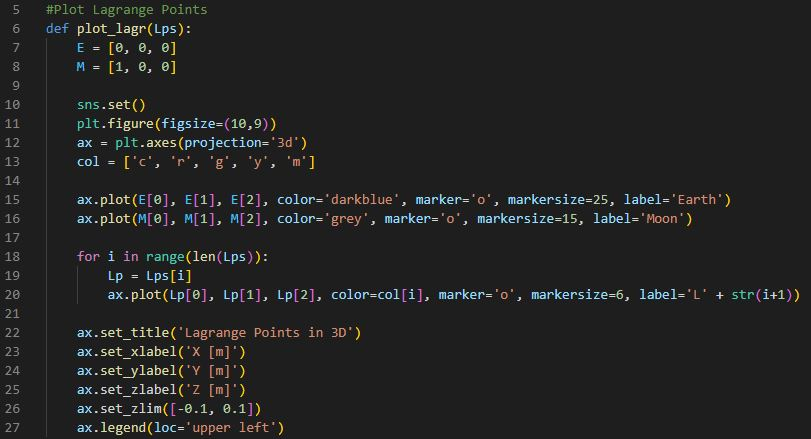
\includegraphics[width=0.95\textwidth]{FIGURES/mil6/codigo/plot_lagr1.JPG}
	\caption{Código función representar en 3D los puntos de Lagrange.}
	\label{plot_lagr1}
\end{figure}

La Figura \ref{plot_lagr2} muestra la función que representa la órbita calculada en las proximidades del punto de Lagrange correspondiente.
\begin{figure}[H]
	\centering
	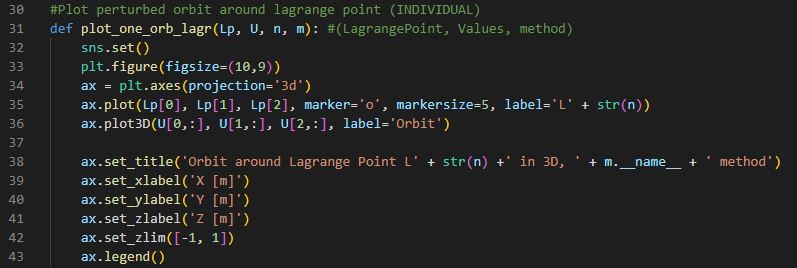
\includegraphics[width=0.95\textwidth]{FIGURES/mil6/codigo/plot_lagr2.JPG}
	\caption{Código función representar en 3D la órbita perturbada alrededor del punto de Lagrange.}
	\label{plot_lagr2}
\end{figure}



\section{Resultados y análisis}
Se ha llevado a cabo una serie de simulaciones para determinar los puntos de Lagrange del sistema Tierra-Luna, así como la estabilidad de estos mismos y el análisis de una órbita en las proximidades de cada uno de los puntos determinados anteriormente.

\subsection{Determinación de los puntos de Lagrange} %OK
\begin{table}[H]
	\centering
	\caption{Puntos de Lagrange Tierra-Luna.}
	\begin{spacing}{1.2}
		\resizebox{0.4\textwidth}{!} {
			\begin{tabular}{|l|l|l|l|}
				\hline 
				Coord. 	& X  		& Y 		& Z \\ \hline \hline
				L1 		& 0.836915 	& 0 		& 0 \\ \hline
				L2 		& 1.155682 	& 0 		& 0 \\ \hline
				L3 		& -1.005063 & 0 		& 0 \\ \hline
				L4 		& 0.487849 	& 0.866025 	& 0 \\ \hline
				L5 		& 0.487849 	& -0.866025 & 0 \\ \hline
			\end{tabular}
		}
	\end{spacing}
	\label{lagr_points} 
\end{table}
La Tabla \ref{lagr_points} muestra los puntos de Lagrange obtenidos con el programa en coordenadas en 3 dimensiones. Dado que los dos cuerpos a estudiar, en este caso la Tierra y la Luna, forman un plano que coincide con el plano XY del sistema de referencia propuesto, la componente en eje Z queda anulada y su valor es cero para todos los puntos obtenidos.

\begin{figure}[H]
	\centering
	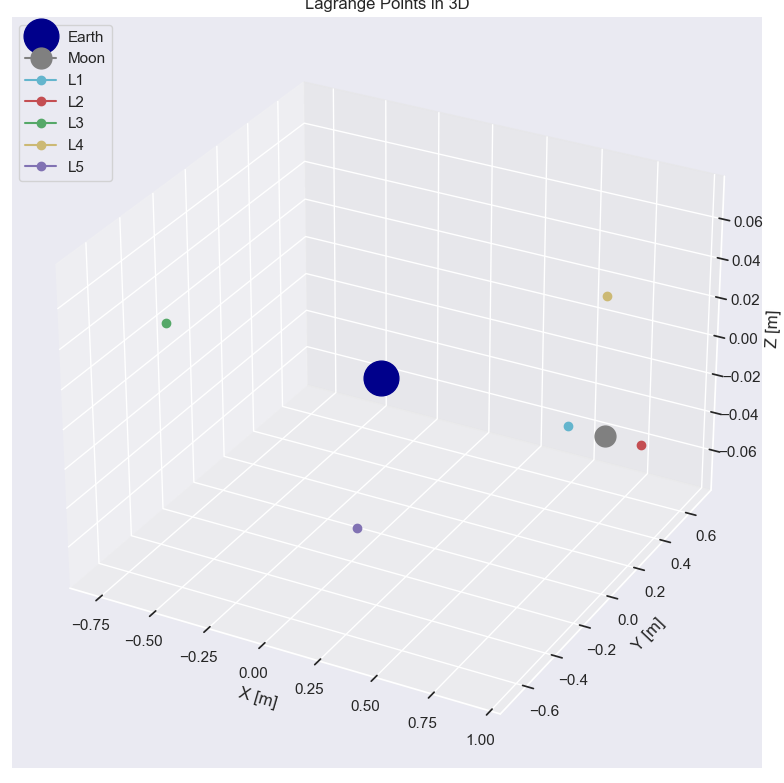
\includegraphics[width=0.90\textwidth]{FIGURES/mil6/langrage_points_erk_3D.png}
	\caption{Representación en 3D de los puntos de Lagrange Tierra-Luna.}
	\label{langrage_points_3D}
\end{figure}
En la Figura \ref{langrage_points_3D} se representan los puntos de Lagrange del sistema Tierra-Luna, así como estos dos cuerpos destacando sobre el resto.


\subsection{Estabilidad de los puntos de Lagrange} %OK
Se han representado en las Figuras \ref{inestable_points} y \ref{stable_points} los autovalores de los distintos puntos de Lagrange en el plano complejo. Puede observarse como los puntos ${L1, L2, L3}$ tienen al menos un autovalor en la parte positiva Real, indicando que es un punto inestable.

Los puntos ${L4, L5}$ también tienen no uno, sino dos autovalores en la región positiva del eje Real, pero como se puede apreciar según la escala, están muy próximos al eje Imaginario. Además este valor se podría asociar a un error de cálculo del propio ordenador. Esto indica que son puntos estables, indicando que para un objeto que se encuentre en las proximidades de este punto su órbita se mantendrá estable en dicho punto y no divergirá. 

%\begin{comment}
\begin{figure}[H]
	\centering
	\subfloat[Autovalores L1]{
		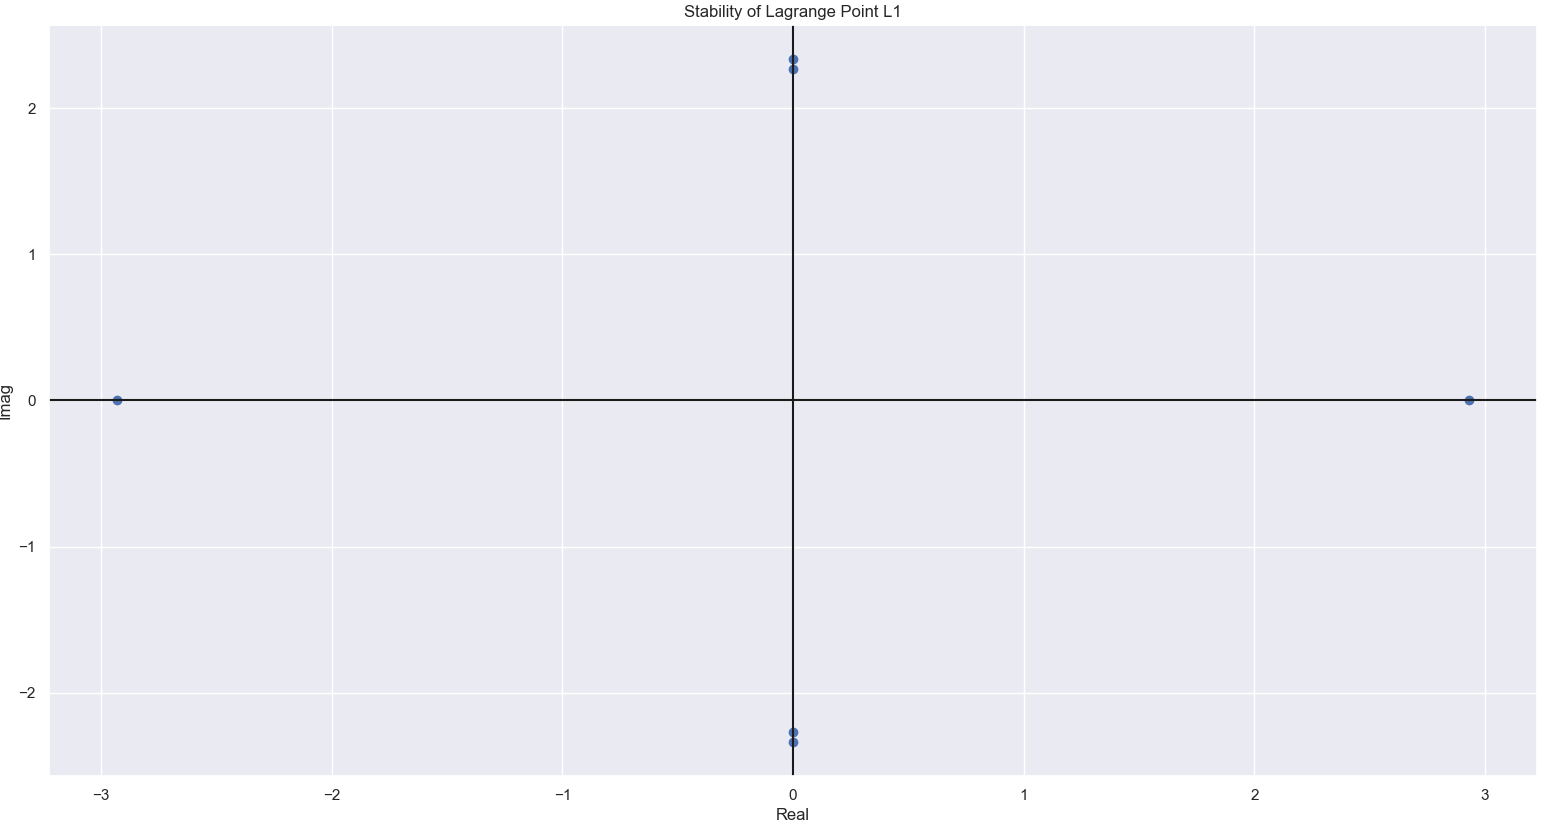
\includegraphics[width=0.33\textwidth]{FIGURES/mil6/stab_L1_erk.png}}
	\subfloat[Autovalores L2]{
		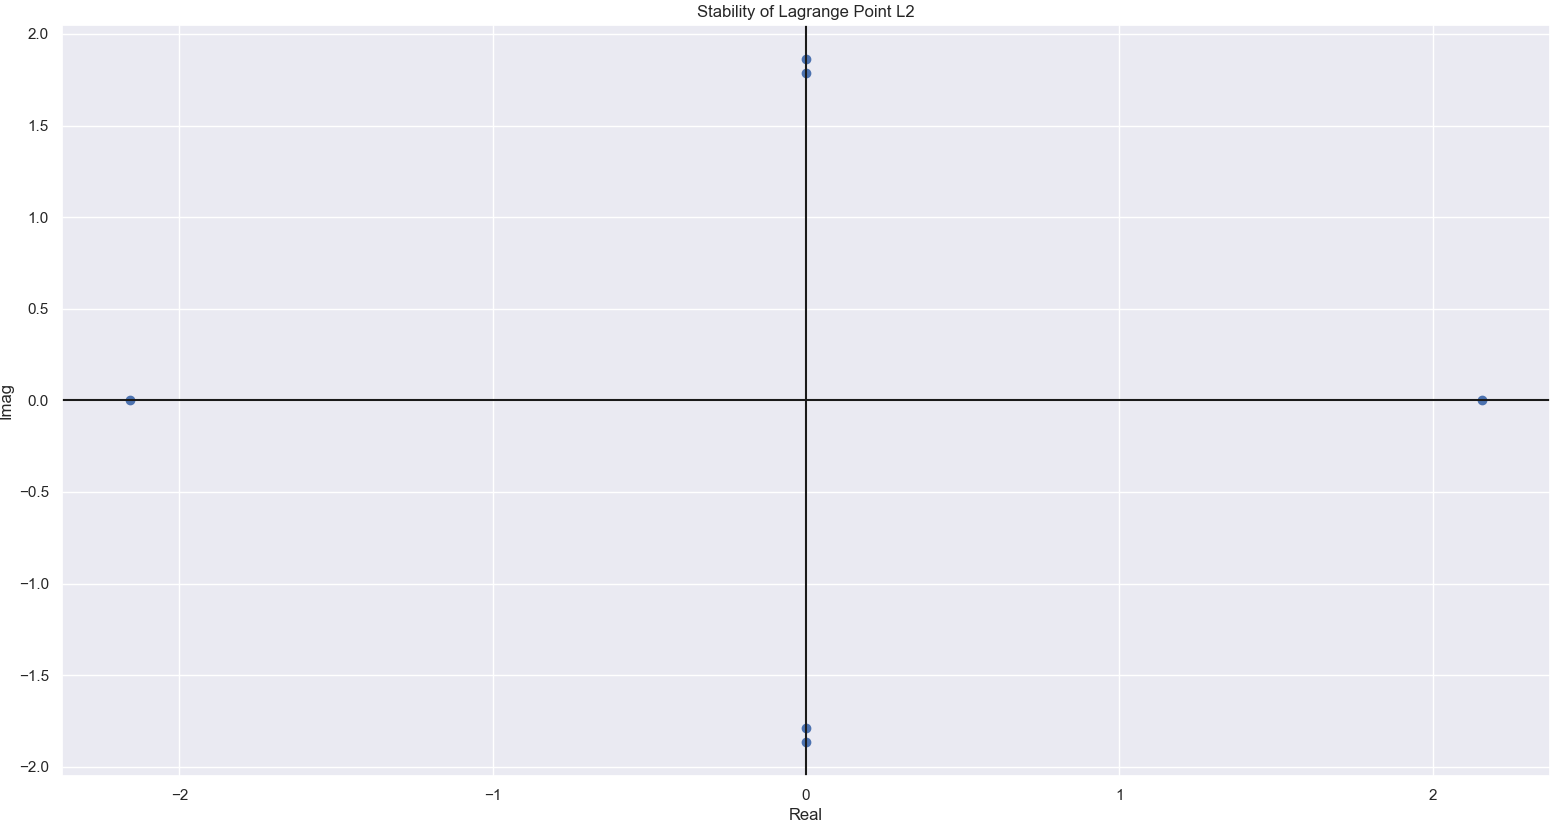
\includegraphics[width=0.33\textwidth]{FIGURES/mil6/stab_L2_erk.png}}
	\subfloat[Autovalores L3]{
		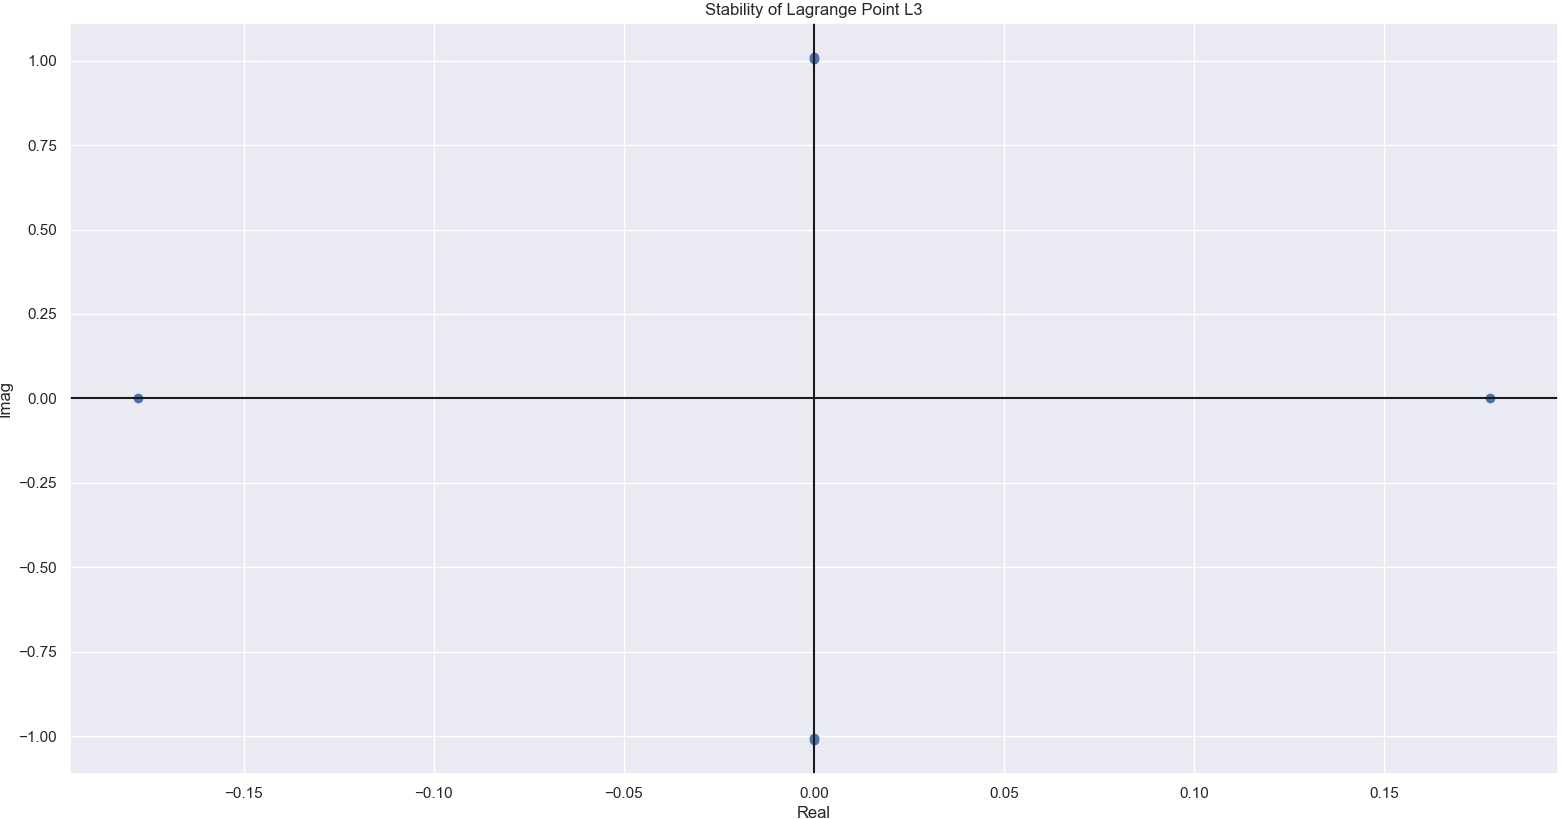
\includegraphics[width=0.33\textwidth]{FIGURES/mil6/stab_L3_erk.png}}

	\caption{Autovalores puntos de Lagrange inestables.}
	\label{inestable_points}
\end{figure}
\begin{figure}[H]
	\centering
	\subfloat[Autovalores L4]{
		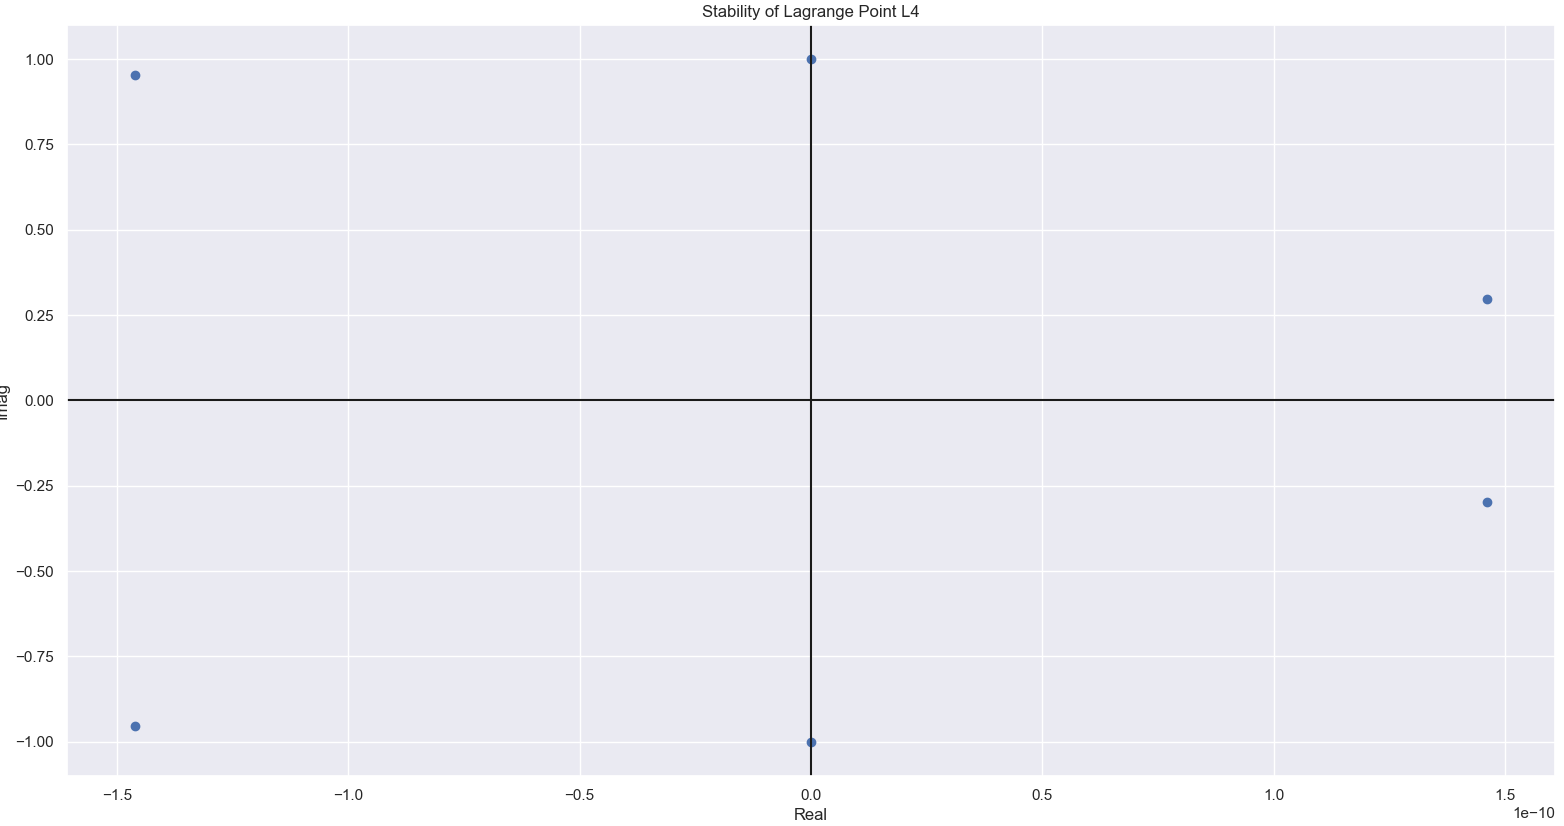
\includegraphics[width=0.49\textwidth]{FIGURES/mil6/stab_L4_erk.png}}
	\subfloat[Autovalores L5]{
		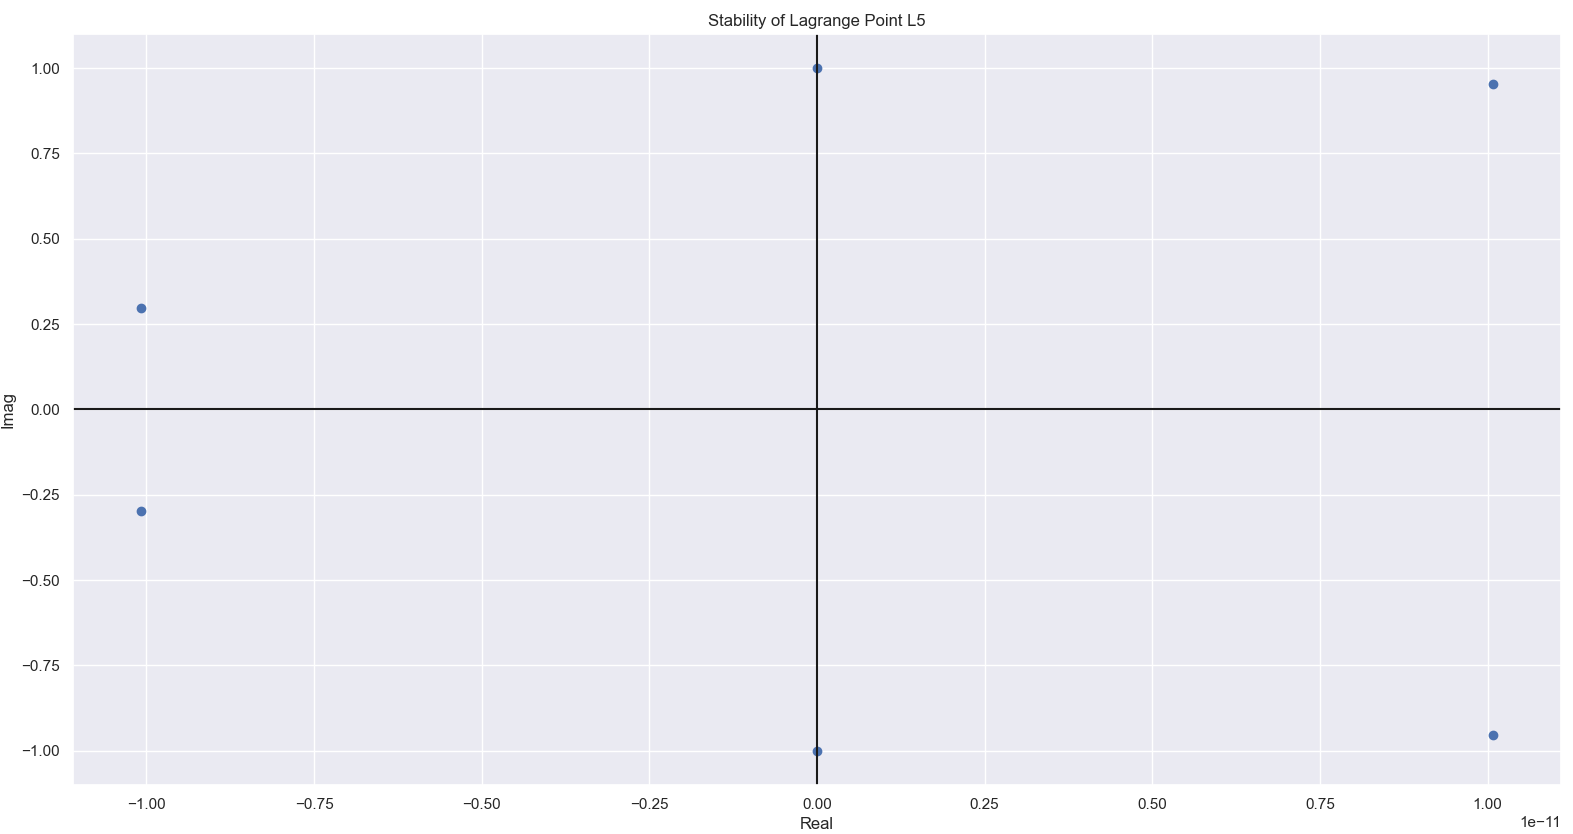
\includegraphics[width=0.49\textwidth]{FIGURES/mil6/stab_L5_erk.png}}
	
	\caption{Autovalores puntos de Lagrange estables.}
	\label{stable_points}
\end{figure}
%\end{comment}

\begin{comment}
\begin{figure}[H]
	\centering
	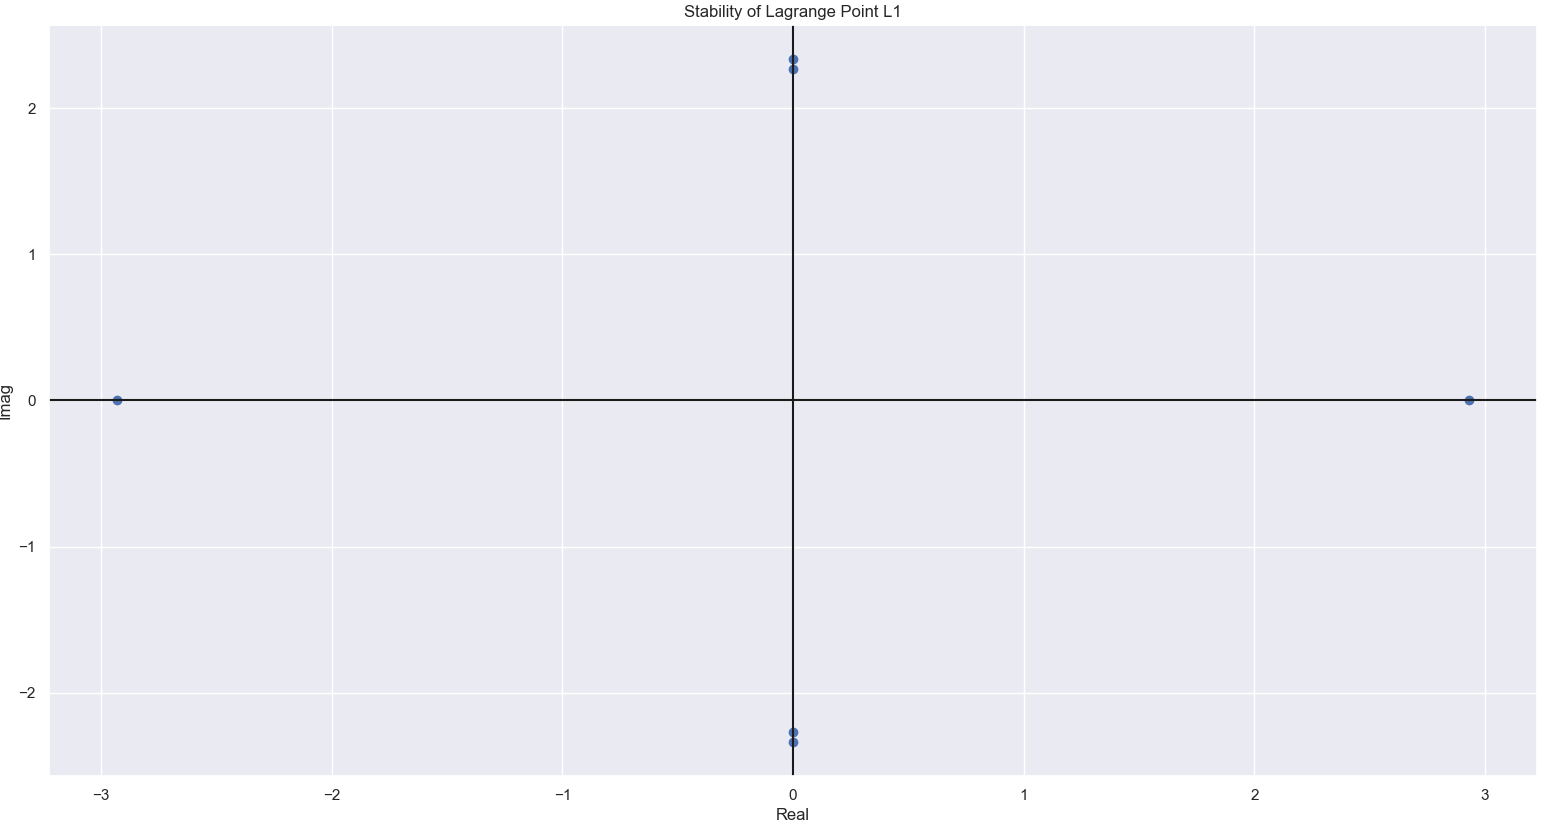
\includegraphics[width=0.8\textwidth]{FIGURES/mil6/stab_L1_erk.png}
	\caption{Raíces L1.}
	\label{stab_L1}
\end{figure}
\begin{figure}[H]
	\centering
	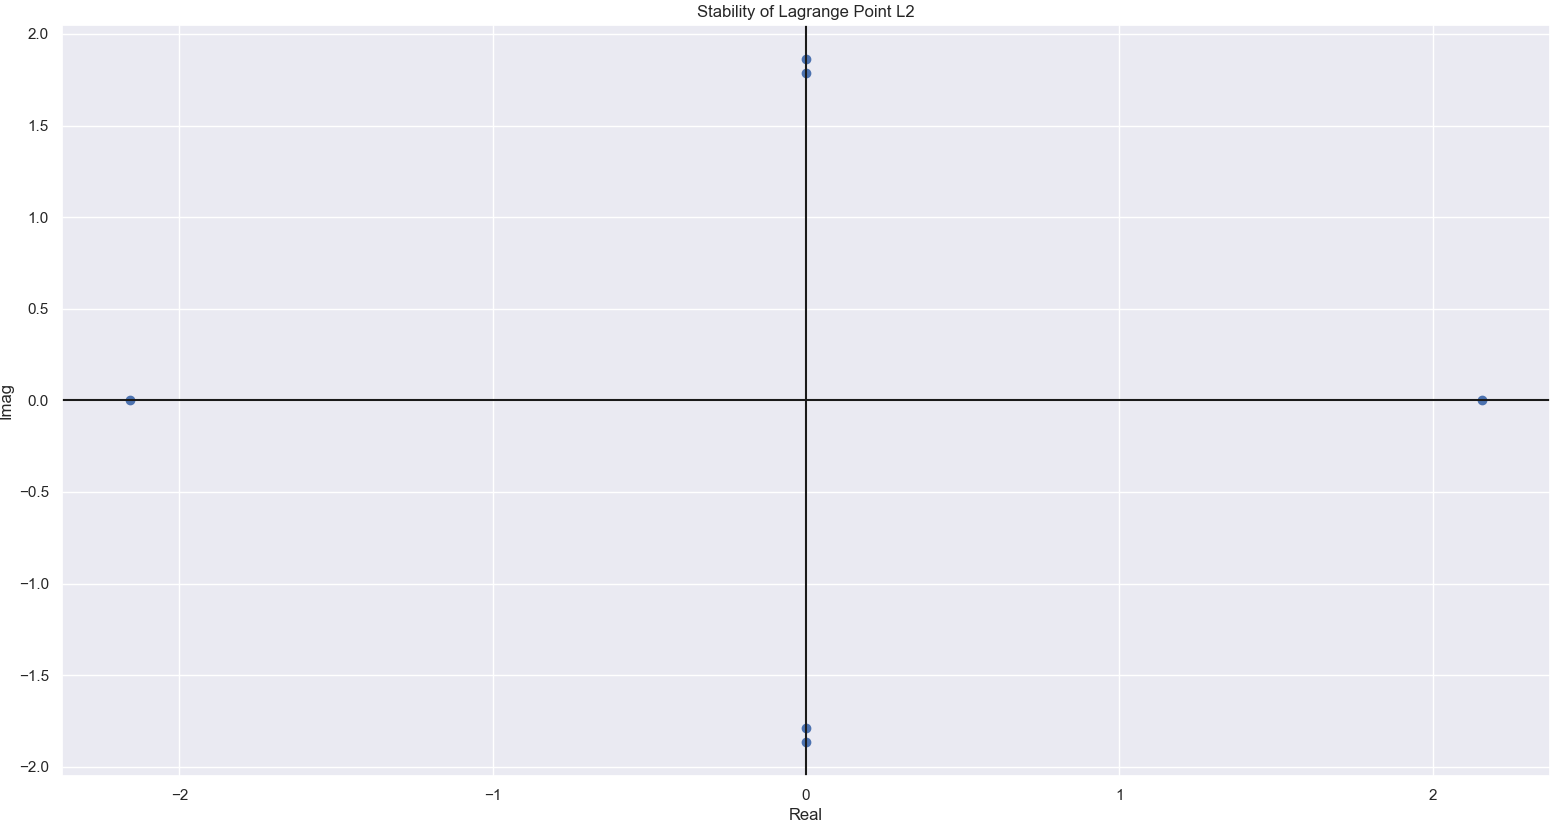
\includegraphics[width=0.8\textwidth]{FIGURES/mil6/stab_L2_erk.png}
	\caption{Raíces L2.}
	\label{stab_L2}
\end{figure}
\begin{figure}[H]
	\centering
	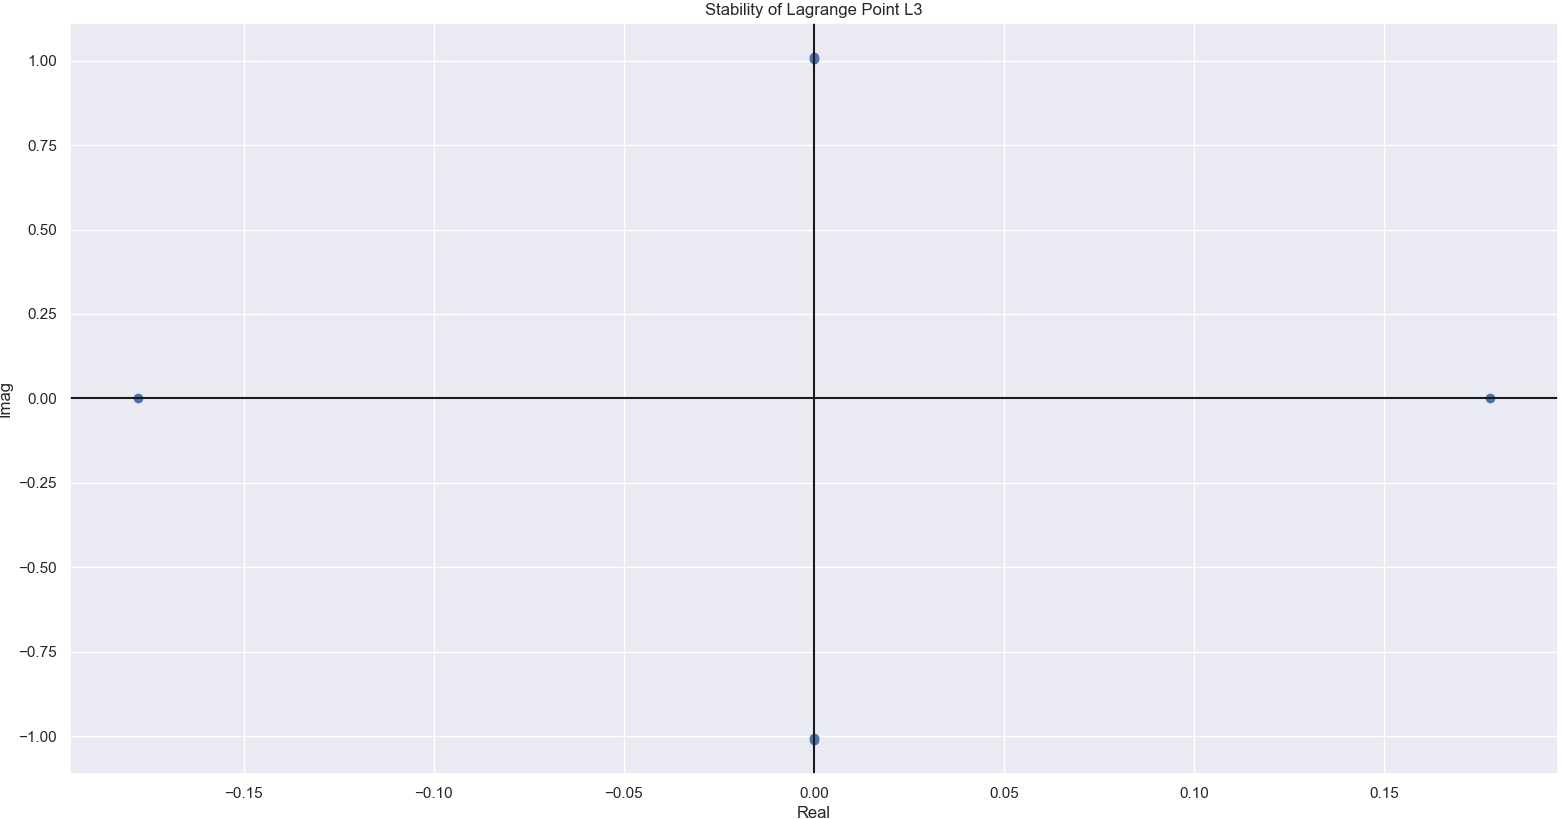
\includegraphics[width=0.8\textwidth]{FIGURES/mil6/stab_L3_erk.png}
	\caption{Raíces L3.}
	\label{stab_L3}
\end{figure}
\begin{figure}[H]
	\centering
	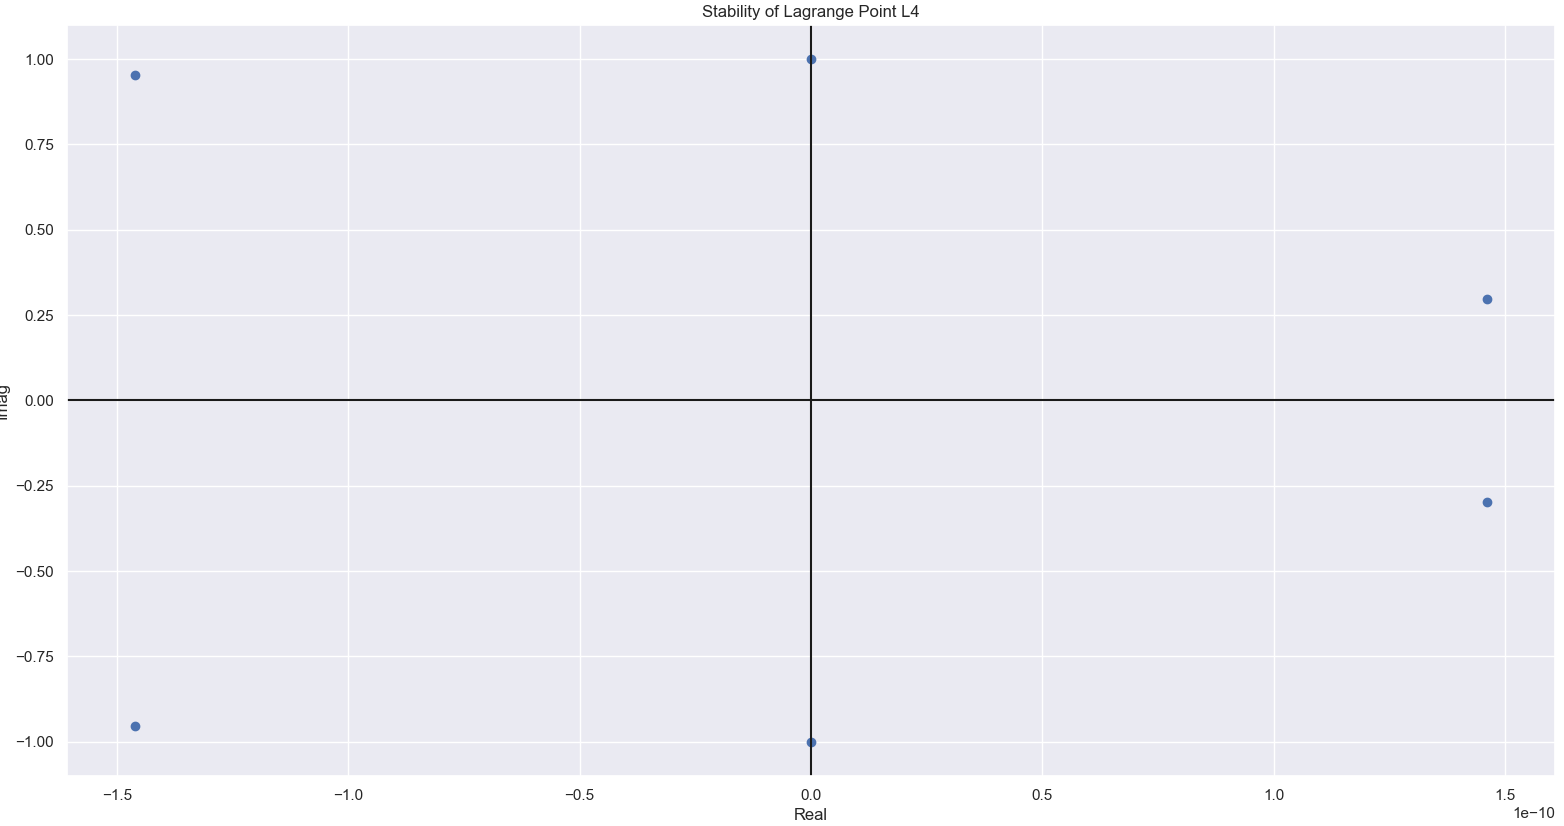
\includegraphics[width=0.8\textwidth]{FIGURES/mil6/stab_L4_erk.png}
	\caption{Raíces L4.}
	\label{stab_L4}
\end{figure}
\begin{figure}[H]
	\centering
	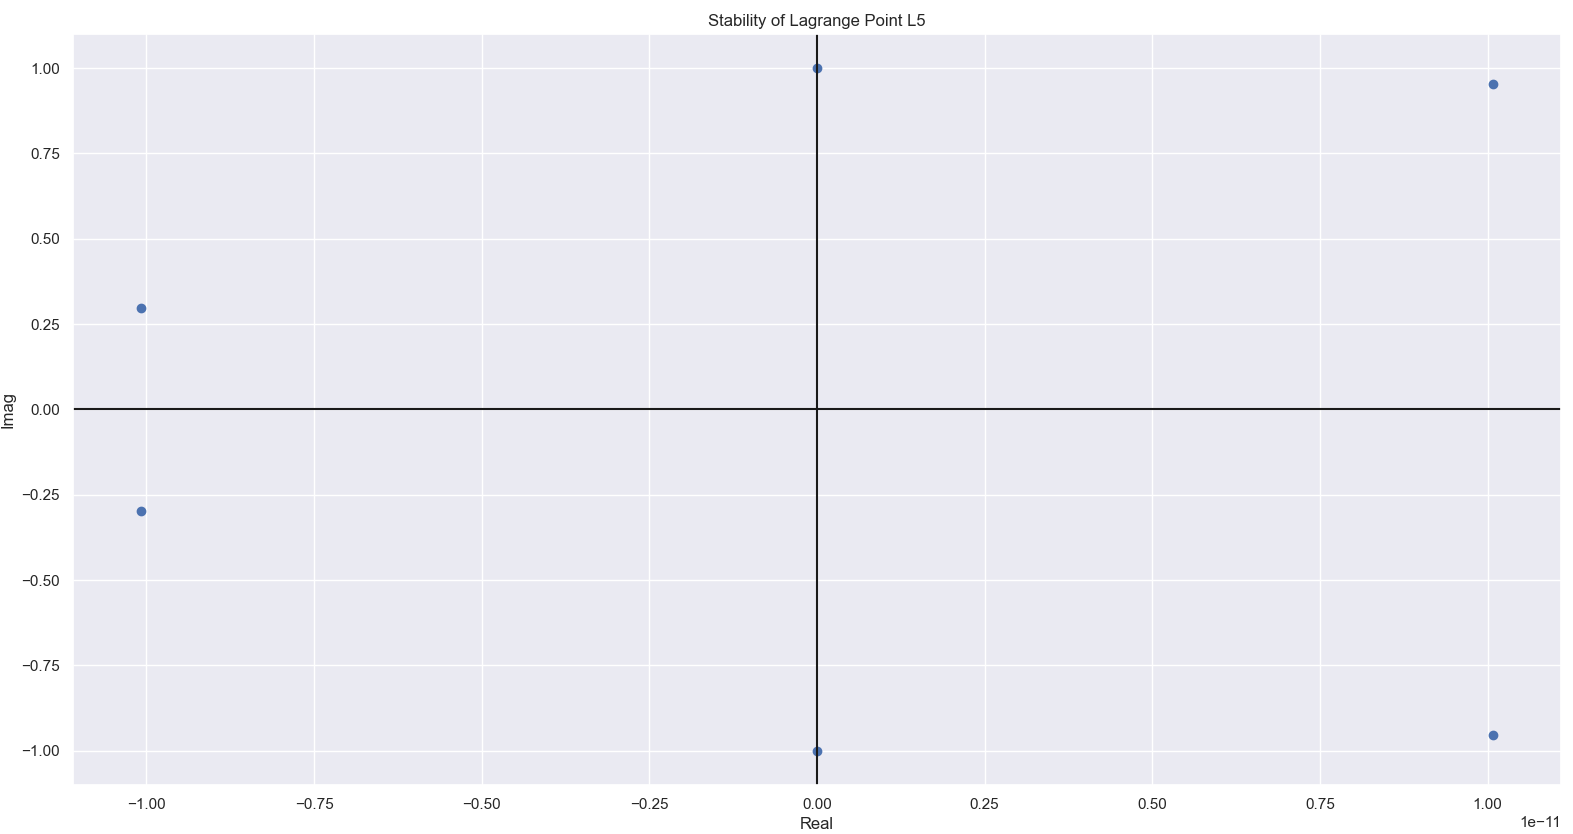
\includegraphics[width=0.8\textwidth]{FIGURES/mil6/stab_L5_erk.png}
	\caption{Raíces L5.}
	\label{stab_L5}
\end{figure}
\end{comment}


\subsection{Órbitas alrededor de los puntos de Lagrange} %OK
En estas simulaciones se ha fijado el tiempo de simulación en 100 segundos y un $\Delta t$ = 0.001 segundos. Se han llevado ha cabo varias simulaciones utilizando varios métodos de resolución numérica.

\subsubsection{Runge-Kutta de alto orden. \textit{RK87}}
Se ha realizado una primera simulación utilizando el esquema numérico RK87 que se ha definido anteriormente.

La Figura \ref{Lptos_orbit_erk_t100} es una representación en 3D del sistema orbital Tierra-Luna, con sus puntos de Lagrange (representados como puntos) y de las órbitas en las proximidades de estos. Las condiciones iniciales de posición para estos cuerpos se han determinado según una función definida en la Figura \ref{main3}, las condiciones de velocidad iniciales son nulas.
\begin{figure}[H]
	\centering
	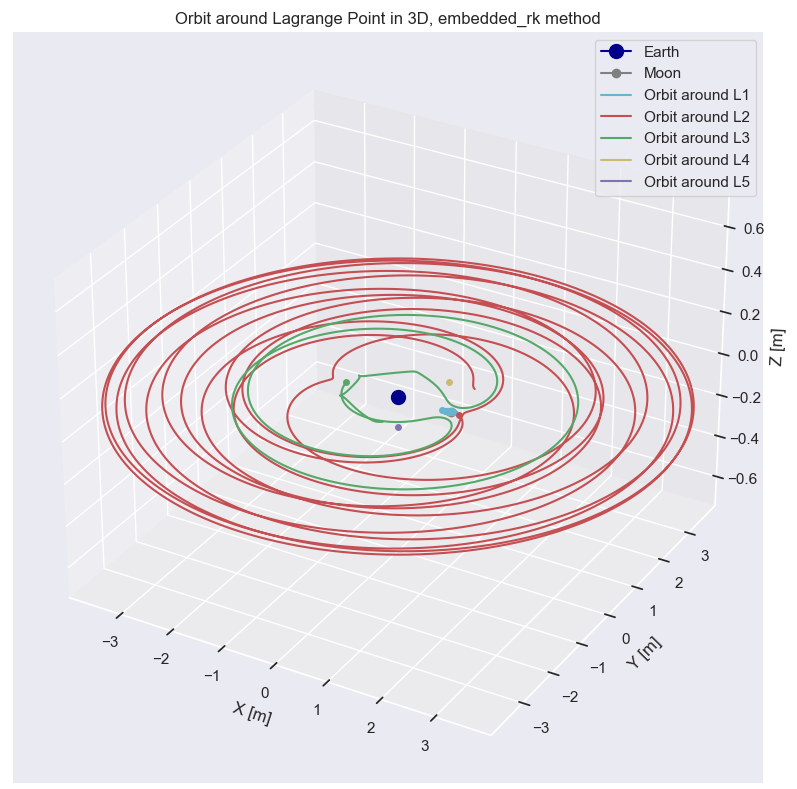
\includegraphics[width=\textwidth]{FIGURES/mil6/Lptos_orbit_erk_t100.png}
	\caption{Representación en 3D de las órbitas sobre los puntos de Lagrange en sistema Tierra-Luna, RK87, $t = 100 s$.}
	\label{Lptos_orbit_erk_t100}
\end{figure}

Las siguientes Figuras representan cada una de las órbitas de los cuerpos alrededor de los puntos de Lagrange de manera individual.

\newcommand\x{0.65}

\begin{figure}[H]
	\centering
	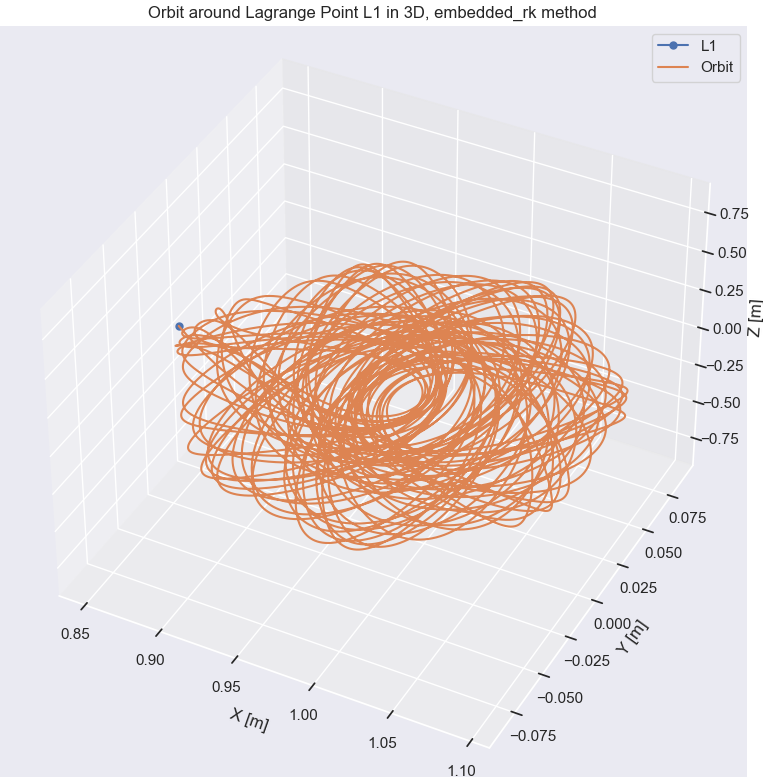
\includegraphics[width=\x\textwidth]{FIGURES/mil6/L1_orbit_erk_t100.png}
	\caption{Órbita en 3D sobre L1, RK87, $t = 100 s$.}
	\label{L1_orbit_erk_t100}
\end{figure}
\begin{figure}[H]
	\centering
	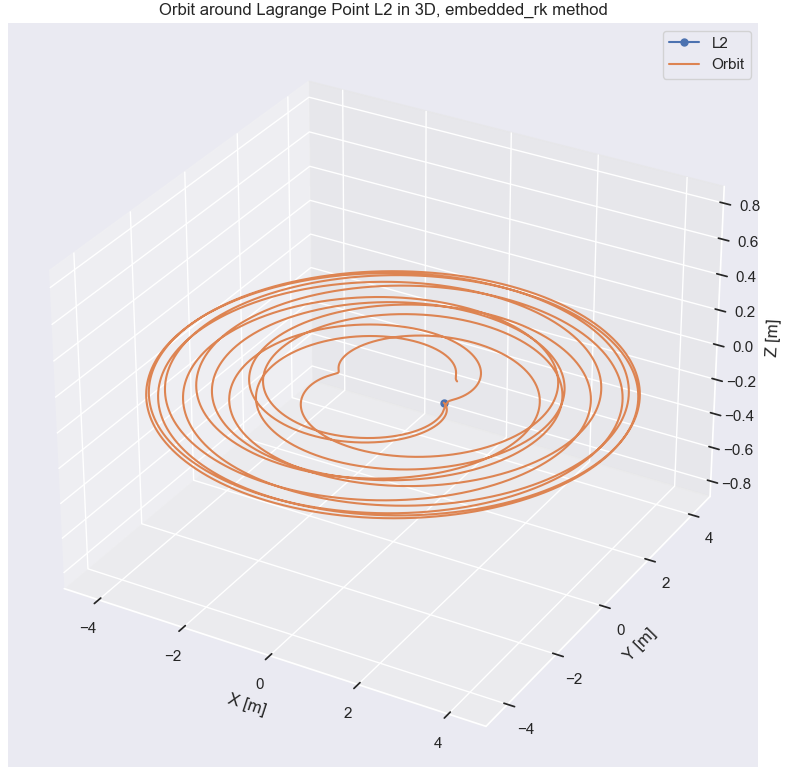
\includegraphics[width=\x\textwidth]{FIGURES/mil6/L2_orbit_erk_t100.png}
	\caption{Órbita en 3D sobre L2, RK87, $t = 100 s$.}
	\label{L2_orbit_erk_t100}
\end{figure}
\begin{figure}[H]
	\centering
	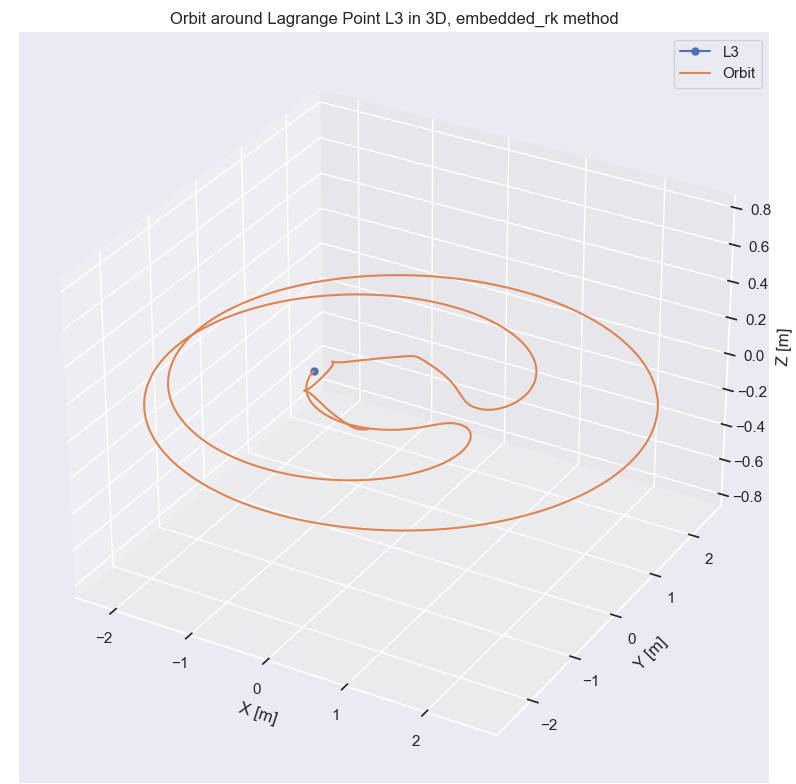
\includegraphics[width=\x\textwidth]{FIGURES/mil6/L3_orbit_erk_t100.png}
	\caption{Órbita en 3D sobre L3, RK87, $t = 100 s$.}
	\label{L3_orbit_erk_t100}
\end{figure}
\begin{figure}[H]
	\centering
	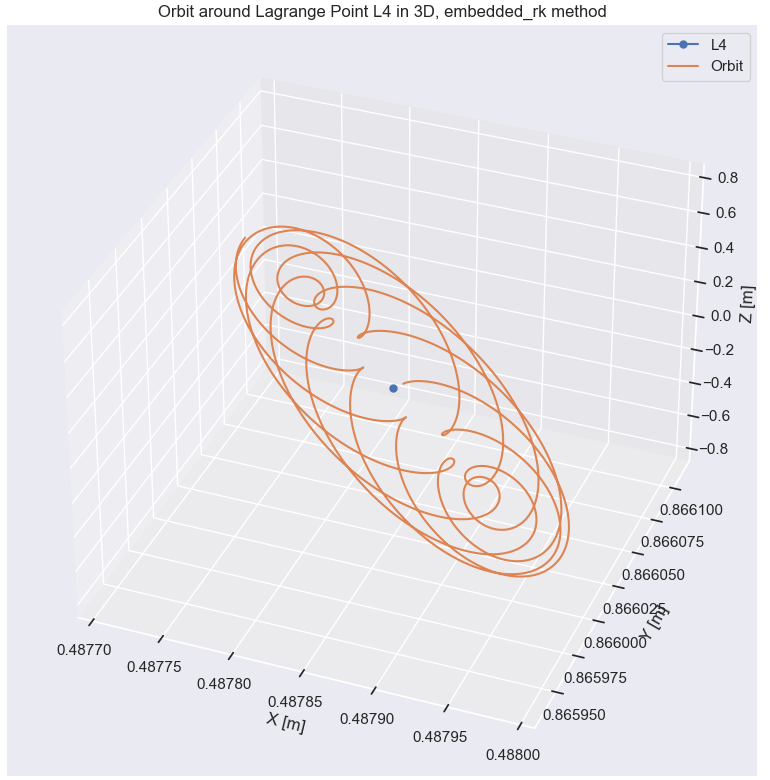
\includegraphics[width=\x\textwidth]{FIGURES/mil6/L4_orbit_erk_t100.png}
	\caption{Órbita en 3D sobre L4, RK87, $t = 100 s$.}
	\label{L4_orbit_erk_t100}
\end{figure}
\begin{figure}[H]
	\centering
	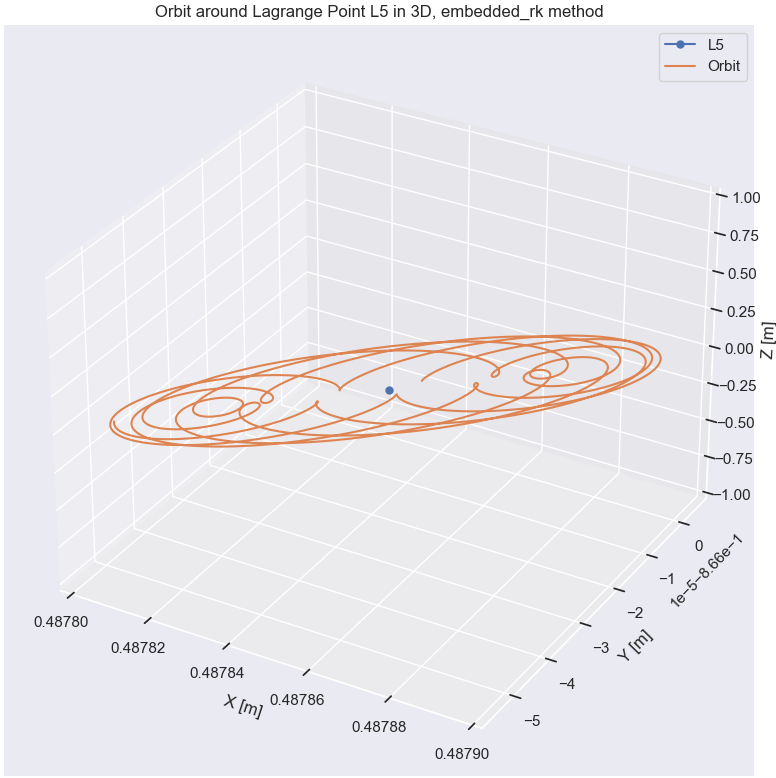
\includegraphics[width=\x\textwidth]{FIGURES/mil6/L5_orbit_erk_t100.png}
	\caption{Órbita en 3D sobre L5, RK87, $t = 100 s$.}
	\label{L5_orbit_erk_t100}
\end{figure}


\subsubsection{Runge-Kutta de orden 4}
A modo de comparación, respecto al nuevo esquema numérico implementado, se ha utilizado para la resolución de las órbitas el método de Runge-Kutta de orden 4 ya implementado en trabajos anteriores. 

A grandes rasgos para las mismas condiciones de simulación (mismos $\Delta t$ y tiempo total) se obtienen unos resultados un poco menos precisos con este método; se puede apreciar en la escala de los ejes de las gráficas obtenidas. 

También es cierto que el tiempo de cómputo es mucho menor con este método. Serviría para la obtención de una primera aproximación de los resultados y luego obtener los resultados más precisos con un método como el RK87.
\begin{figure}[H]
	\centering
	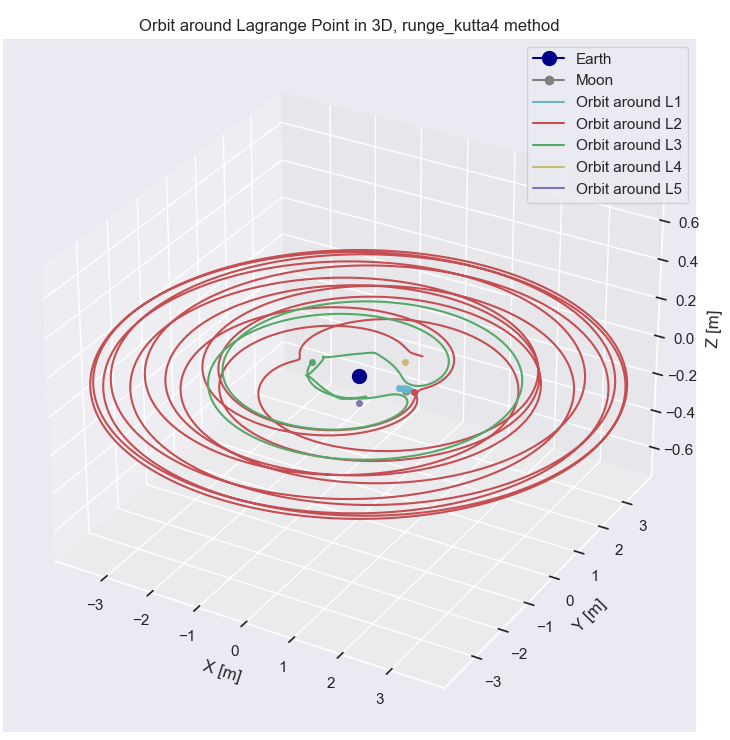
\includegraphics[width=\textwidth]{FIGURES/mil6/Lptos_orbit_rk4_t100.png}
	\caption{Representación en 3D de las órbitas sobre los puntos de Lagrange en sistema Tierra-Luna, RK4, $t = 100 s$.}
	\label{Lptos_orbit_rk4_t100}
\end{figure}

\begin{figure}[H]
	\centering
	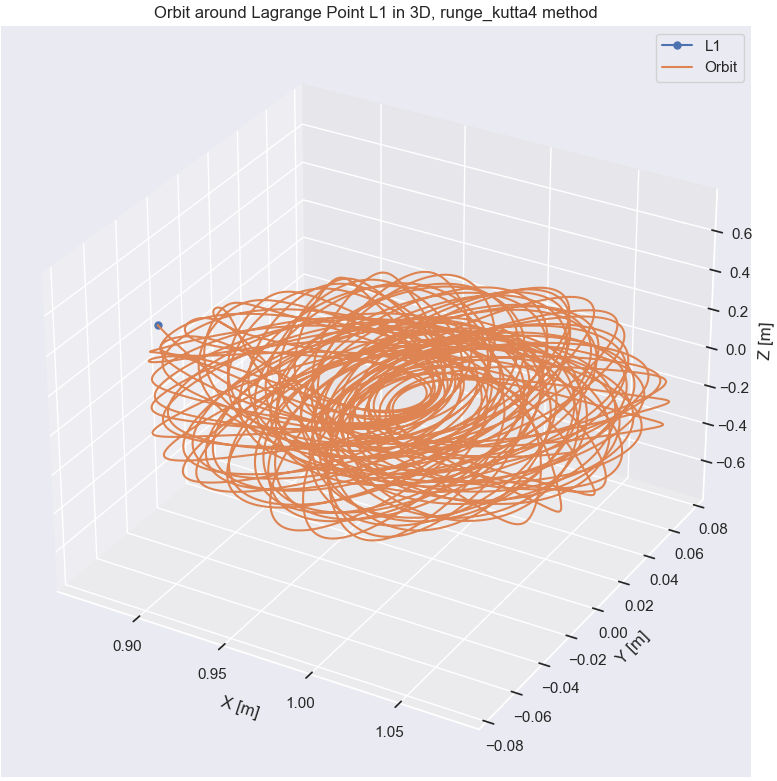
\includegraphics[width=\x\textwidth]{FIGURES/mil6/L1_orbit_rk4_t100.png}
	\caption{Órbita en 3D sobre L1, RK4, $t = 100 s$.}
	\label{L1_orbit_rk4_t100}
\end{figure}
\begin{figure}[H]
	\centering
	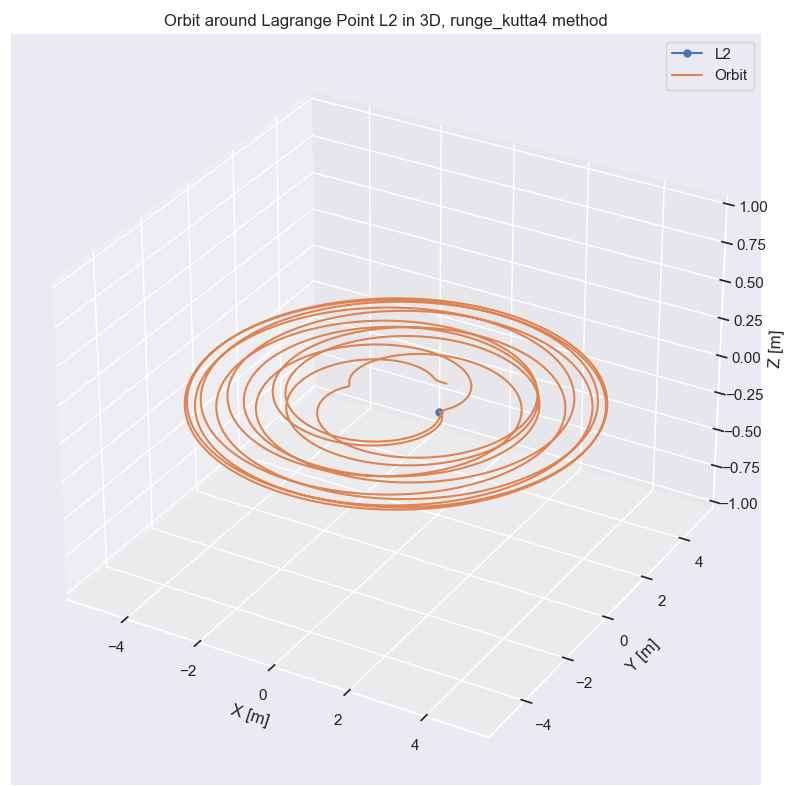
\includegraphics[width=\x\textwidth]{FIGURES/mil6/L2_orbit_rk4_t100.png}
	\caption{Órbita en 3D sobre L2, RK4, $t = 100 s$.}
	\label{L2_orbit_rk4_t100}
\end{figure}
\begin{figure}[H]
	\centering
	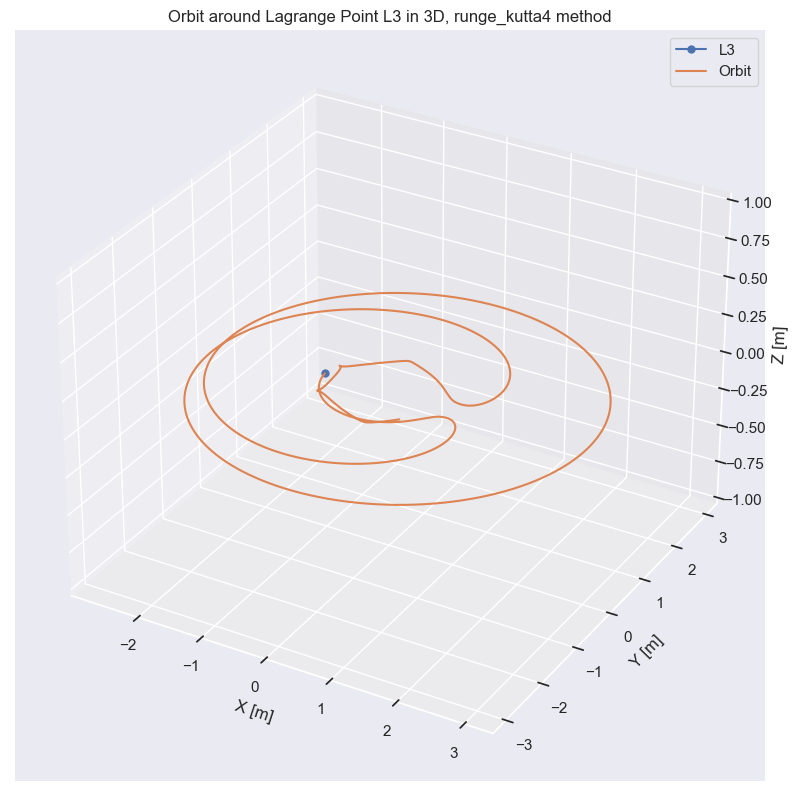
\includegraphics[width=\x\textwidth]{FIGURES/mil6/L3_orbit_rk4_t100.png}
	\caption{Órbita en 3D sobre L3, RK4, $t = 100 s$.}
	\label{L3_orbit_rk4_t100}
\end{figure}
\begin{figure}[H]
	\centering
	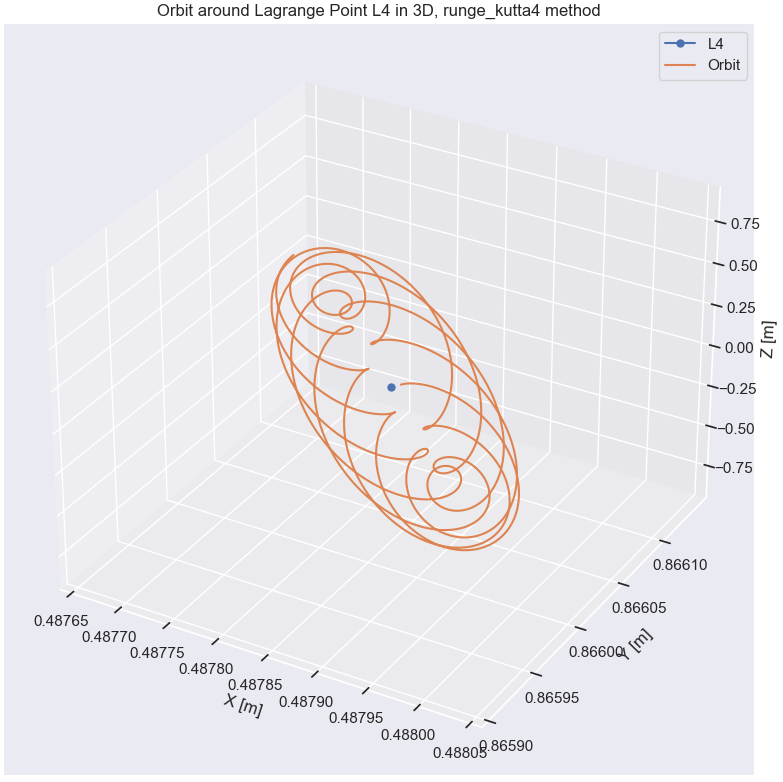
\includegraphics[width=\x\textwidth]{FIGURES/mil6/L4_orbit_rk4_t100.png}
	\caption{Órbita en 3D sobre L4, RK4, $t = 100 s$.}
	\label{L4_orbit_rk4_t100}
\end{figure}
\begin{figure}[H]
	\centering
	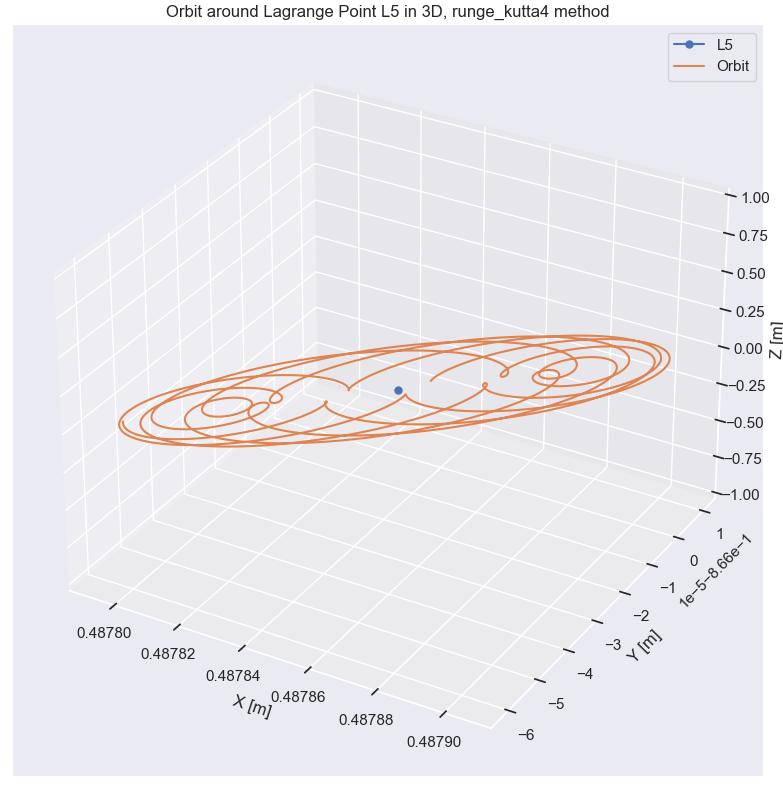
\includegraphics[width=\x\textwidth]{FIGURES/mil6/L5_orbit_rk4_t100.png}
	\caption{Órbita en 3D sobre L5, RK4, $t = 100 s$.}
	\label{L5_orbit_rk4_t100}
\end{figure}

\paragraph{Simulaciones con otros métodos de resolución numérica}
Se han simulado las órbitas con otros métodos ya implementados en anteriores trabajos, como lo son el Método de Euler, Crank-Nicolson y Leap-Frog. 

Los resultados no se muestran en este informe puesto que algunos de ellos (Euler, Euler inverso y Leap-Frog), incluso con $\Delta t$ pequeños, el resultado que se obtiene es una divergencia de los cuerpos a los pocos segundos de simulación. Con el método de Crank-Nicolson se pueden obtener buenos resultados pero aún así divergen cuando se simula durante tiempos mayores a 100 segundos.



\section{Conclusiones} %OK
Cabe destacar el tiempo de procesado que se necesita para realizar las simulaciones utilizando un método como es el \textit{RK87} de alto orden en comparación con los métodos que ya se habían implementado en los anteriores trabajos, para las mismas condiciones de tiempo de simulación y de paso temporal $\Delta t$. Por el contrario se obtienen unos resultados mucho más precisos con el método RK87 que con el resto de métodos implementados.

Una buena extensión de este trabajo sería la de poder realizar el cálculo de las órbitas de cada punto de Lagrange de forma paralela. De esta forma se aprovecharía mejor la potencia del PC y se reduciría el tiempo de computo. 

\end{document}
